\documentclass[cyan]{elegantnote}
\author{Yuyang Songsheng}
\email{songshengyuyang@gmail.com}
\zhtitle{物理}
\entitle{Physics}
\version{1.00}
\myquote{Do not ask what it is. Ask what you can say about it.}
\logo{logo.jpg}
\cover{cover.pdf}
%green color
   \definecolor{main1}{RGB}{210,168,75}
   \definecolor{seco1}{RGB}{9,80,3}
   \definecolor{thid1}{RGB}{0,175,152}
%cyan color
   \definecolor{main2}{RGB}{239,126,30}
   \definecolor{seco2}{RGB}{0,175,152}
   \definecolor{thid2}{RGB}{236,74,53}
%cyan color
   \definecolor{main3}{RGB}{127,191,51}
   \definecolor{seco3}{RGB}{0,145,215}
   \definecolor{thid3}{RGB}{180,27,131}


\usepackage{makecell}
\usepackage{lipsum}
\usepackage{amssymb}
\usepackage{float}
\usepackage{wrapfig}
\usepackage{latexsym}
\usepackage{hyperref}
\usepackage{feynmf}
\usepackage{exscale}
\usepackage{relsize}
\usepackage{bm}%bold math, for vector


\begin{document}
\maketitle
\tableofcontents
\chapter{The formulation of Classical Mechanics}
\section{Lagrangian Formulation}
\[S=\int_{t_1}^{t_2}L(q_i,\dot{q_i},t)dt, \ \ \ \ \delta q_i(t_1) = \delta q_i(t_2) = 0\]
\[\delta S=0 \rightarrow \frac{d}{dt}(\frac{\partial L}{\partial \dot{q_i}}) - \frac{\partial L}{\partial q_i}=0\]

\begin{enumerate}
\item If we transform the coordinates $q$ to the $Q$ as $q = q(Q,t)$, the new Lagrangian will be
\[\bar{L}(Q,\dot{Q},t) \equiv L(q(Q,t),\dot{q}(Q,\dot{Q},t),t)\]
We can verify that
\[\frac{d}{dt}\frac{\partial \bar{L}}{\partial \dot{Q}} - \frac{\partial \bar{L}}{\partial Q} = 0\]
\item If $L_1 = L + \frac{d}{dt} f(q,t)$, then $L$ and $L_1$ is equivalent and will generate the same dynamical equation.
\end{enumerate}

\begin{example}
\begin{enumerate}
\item The form of Lagrangian for an isolated system of particles in inertial frame:
\[L=\sum_a \frac{1}{2}m_a v_a^2 -U(\bm{r}_1,\bm{r}_2,\cdots,)\]
The equation of motion is
\[m_i \ddot{\bm{r}}_i = -\nabla_{\bm{r}_i} U\]
To get the form of Lagrangian for a system of interacting particles, we must assume:
\begin{itemize}
\item Space and time are homogeneous and isotropic in inertial frame;
\item Galileo's relativity principle and Galilean transformation;
\item Spontaneous interaction between particles;
\end{itemize}
\item Consider a reference frame $K$. Suppose the $K$ is moving with the velocity $\bm{V}(t)$ and  rotating with angular velocity $\bm{\Omega}$  relative to the inertial reference frame. We use the coordinates of the mass point in $K$ as general coordinates, i.e. $\bm{r} = (x_k,y_k,z_k)$. Then the Lagrangian of the mass point will be
\[L = \frac{1}{2}m\bm{v}^2 + m\bm{v}\cdot(\bm{\Omega}\times\bm{r})+\frac{m}{2}(\bm{\Omega}\times\bm{r})^2 - m\dot{\bm{V}}\cdot\bm{r}-U\]
The equation of motion will be
\[m\frac{d\bm{v}}{dt} = -\frac{\partial U}{\partial \bm{r}} - m\dot{\bm{V}} + m(\bm{r} \times \dot{\bm{\Omega}}) + 2m(\bm{v} \times \bm{\Omega}) + m[\bm{\Omega}\times(\bm{r} \times \bm{\Omega})]\]
\end{enumerate}
\end{example}

\section{Symmetry and Conservation Laws(1)}
\begin{newthem}[Nother's theorem]
For $q_i \to q_i+\delta q_i$ and $L \to L+\delta L$, if $\delta L= \frac{d f(q,\dot{q},t)}{dt}$,then we get
\[\frac{d}{dt}(\sum_i p^i \delta q_i-f)=0 \ \ \ (p^i=\frac{\partial L}{\partial \dot{q_i}})\]
\end{newthem}
\begin{example}
For an isolated system of particles in inertial frame,\\ 
$\delta L = 0$ when $\delta \bm{r}_i \rightarrow \bm{r}_i + \delta \bm{a}$, so
\[\frac{d}{dt} (\sum_i \bm{p}_i) = 0\]
$\delta L = 0$ when $\delta \bm{r}_i \rightarrow \bm{r}_i + \bm{r}_i \times \delta \bm{\theta}$, so
\[\frac{d}{dt} (\sum_i \bm{r}_i \times \bm{p}_i) = 0\]
\end{example}

\paragraph{Homogeneity of time}
If $\frac{\partial L}{\partial t}=0$,then we get
\[\frac{dE}{dt}=0 \ \ \ (E=\sum_i \dot{q_i}p^i-L)\]

\section{Hamilton formulation}
\[p^i = \frac{\partial L}{\partial \dot{q_i}}\]
\[H(q,p,t)=\sum_i p^i \dot{q_i}-L\]
\[\dot{p^i}=-\frac{\partial H}{\partial q_i} \quad \dot{q_i}=\frac{\partial H}{\partial p^i}\]
\begin{example}
 For an isolated system of particles in inertial frame, 
\[\bm{p}_i = m_i \bm{v}_i\]
\[H(q,p,t)=\sum_i \frac{p_i^2}{2m} + U(\bm{r}_1,\bm{r}_2,\cdots)\]
\[\dot{\bm{p}}_i =-\nabla_{\bm{r}_i} U \quad \dot{\bm{r}}_i = \frac{\bm{p}_i}{m_i}\]
\end{example}
 
\subsection{Poisson Brackets}
First, we assume the bracket operation has the following properties:
\[ \left[f,g\right]=-\left[g,f\right] \]
\[\left[\alpha_1 f_1+\alpha_2 f_2,\beta_1 g_1+\beta_2 g_2\right]=\alpha_1 \beta_1\left[f_1,g_1\right]
+\alpha_1 \beta_2\left[f_1,g_2\right]+\alpha_2 \beta_1\left[f_2,g_1\right]+\alpha_2 \beta_2\left[f_2,g_2\right]\]
\[\left[f_1 f_2,g_1 g_2\right]=f_1\left[f_2,g_1\right]g_2+f_1 g_1\left[f_2,g_2\right]+g_1\left[f_1,g_2\right]f_2 +\left[f_1,g_1\right]g_2 f_2 \]
\[\left[f,\left[g,h\right]\right]+\left[g,\left[h,f\right]\right]+\left[h,\left[f,g\right]\right]=0\]
Here, $f,g,h$ are functions of $p^i,q_i,t$.
Then, we assume that
\[\left [q_i,p^k\right ]=\delta^{k}_{i}\]
we can derive that 
\[ \left[f,g\right]=\sum_k(\frac{\partial f}{\partial q_k} \frac{\partial g}{\partial p^k} - \frac{\partial f}{\partial p^k} \frac{\partial g}{\partial q_k}  )\]
So the Hamilton equation can be written as
\[\dot{p^i}=\left[ p^i,H \right] \ \ \ \ \dot{q_i}=\left[ q_i,H \right]\]
And we can also get
\[\frac{df}{dt} = [f,H] + \frac{\partial f}{\partial t} \quad \frac{d}{dt} [f,g] = [\frac{df}{dt},g] + [f,\frac{dg}{dt}]\]
\begin{example}
 For an isolated system of particles in inertial frame, 
\[[r_{ia},p_{jb}] = \delta_{ab} \delta_{ij}\]
we define $l_a = \epsilon_{abc} r_{a} p_{b}$, then
\[[l_a,r_b] = \epsilon_{abc}r_c \quad [l_a,p_b] = \epsilon_{abc}p_c \quad [l_a,l_b] = \epsilon_{abc}l_c\]
\end{example}

\subsection{Canonical transformations}
In Hamiltonian mechanics, a canonical transformation is a change of canonical coordinates that preserves the form of Hamilton's equations (that is, the new Hamilton's equations resulting from the transformed Hamiltonian may be simply obtained by substituting the new coordinates for the old coordinates), although it might not preserve the Hamiltonian itself. 
\[Q_i = Q_i(p,q,t) \quad P_i=P_i(p,q,t)\]
\[\dot{Q}_i = \frac{\partial H'}{\partial P_i} \quad \dot{P}_i = -\frac{\partial H'}{\partial Q_i}\]

\begin{newprop}[Canonical condition]
If $(q_i,p^i,H) \to (Q_i,P^i,H)$ is a canonical transformation, then there exists a generating function $F(q_i,Q_i,t)$ satisfying that
\[\sum_i p^i\dot{q}_i-H(p^i,q_i) = \sum_i P^i\dot{Q_i} - H'(Q_i,P^i) + \frac{dF}{dt}\]
\end{newprop}

Applying Legendre transformation, we can get four kinds of generating function. 
\begin{enumerate}
\item \[\frac{dF}{dt} = \sum_i p^i \dot{q}_i - \sum_i P^i \dot{Q}^i + (H'-H)\]
Assume $\Phi(q_i,Q_i,t) = F$, so
\[p^i = \frac{\partial \Phi}{\partial q_i} \quad P^i = -\frac{\partial \Phi}{\partial Q_i} \quad H' = H + \frac{\partial \Phi}{\partial t}\]

\item \[\frac{d}{dt}(F+\sum_i P^i Q_i) = \sum_i p^i \dot{q}_i + \sum_i Q_i \dot{P}^i + (H'-H)\]
Assume $\Phi(q_i,P^i,t) = F + \sum_i P^i Q_i$, so
\[p^i = \frac{\partial \Phi}{\partial q_i} \quad Q_i = \frac{\partial \Phi}{\partial P^i} \quad H' = H + \frac{\partial \Phi}{\partial t}\]

\item \[\frac{d}{dt}(F-\sum_i p^i q_i) = -\sum_i q_i \dot{p}^i - \sum_i P^i \dot{Q}_i + (H'-H)\]
Assume $\Phi(p^i,Q_i,t) = F - \sum_i p^i q_i$, so
\[q_i = -\frac{\partial \Phi}{\partial p^i} \quad P^i = -\frac{\partial \Phi}{\partial Q_i} \quad H' = H + \frac{\partial \Phi}{\partial t}\]

\item \[\frac{d}{dt}(F+\sum_i P^i Q_i-\sum_i p^i q_i) = -\sum_i q_i \dot{p}^i + \sum_i Q_i \dot{P}^i + (H'-H)\]
Assume $\Phi(p^i,P^i,t) = F+\sum_i P^i Q_i-\sum_i p^i q_i$, so
\[q_i = -\frac{\partial \Phi}{\partial p^i} \quad Q_i = \frac{\partial \Phi}{\partial P^i} \quad H' = H + \frac{\partial \Phi}{\partial t}\]
\end{enumerate}

\begin{newthem}[The invariance of Poisson Bracket]
Suppose that $(q,p,H) \to (Q,P,H')$ is a canonical transformation and $f(q,p,t) = F(Q,P,t)$, $g(q,p,t) = G(Q,P,t)$, then
\[[f,g]_{q,p} = [F,G]_{Q,P}\]
\end{newthem}
As a result, the condition for canonical transformation can also be stated as
\[[Q_i,Q_j]_{q,p} = 0 \quad [P^i,P^j]_{p,q} = 0 \quad [Q_i,P^j]_{q,p} = \delta_i^j\]

\subsection{Evolution as canonical transformations}
Let $q_t$,$p_t$ be the values of the canonical variables at time $t$, and $q_{t+\tau}$,$p_{t+\tau}$ their values at another time $t+\tau$. The latter are some functions of the former:
\[q_{t+\tau} = q(q_t,p_t,t,\tau) \quad p_{t+\tau} = p(q_t,p_t,t,\tau)\]
If these formulae are regarded as a transformation from the variables $q_t$,$p_t$ to $q_{t+\tau}$, $p_{t+\tau}$, then this transformation is canonical. This is evident from the
expression
\[dS = p_t dq_t + p_{t+\tau} dq_{t+\tau} -(H_{t+\tau}-H_t)dt\]
for the differential of the action $S(q_t,q_{t+\tau},t,\tau)$, taken along the true path, passing through the points $q$, and $q_{t+\tau}$ at times $t$ and $t+\tau$ for a given $\tau$. $-S$ is the generating function of the transformation. So we have the following communication relation
\[[q_{i\,t+\tau},q_{j\,t+\tau}]_{q_t,p_t} = 0 \quad [p^i_{t+\tau},p^j_{t+\tau}]_{q_t,p_t} = 0 \quad [q_{i\,t+\tau},p^j_{t+\tau}]_{q_t,p_t} = \delta_i^j\]

\subsection{Liouville's theorem}
\begin{newlemma}
Let $D$ be the Jacobian of the canonical transformation 
\[\frac{\partial(Q_1,\cdots,Q_s,P^1,\cdots,P^s)}{\partial(q_1,\cdots,q_s,p^1,\cdots,p^s)}\]
Then we have
\[D=1\]
\end{newlemma}

\begin{newthem}[Liouville's theorem]
The phase-space distribution function is constant along the trajectories of the system
\end{newthem}

\begin{newproof}
The phase volume is invariant under canonical transformation.The change in $p$ and $q$ during the motion can be regarded as a canonical transformation. Suppose that each point in the region of phase space moves in the course of time in accordance with the equations of motion of the mechanical system. The region as a whole therefore moves also, but its volume remains unchanged.
\end{newproof}

\section{Symmetry and Conservation Laws(2)}
Suppose $g$ is a function of $p$ and $q$. If the transformation of $q$ and $p$ can be described as
\[q \rightarrow q + \epsilon [q,g]\]
\[p \rightarrow p + \epsilon [p,g]\]
We can prove that 
\[H \rightarrow H + \epsilon[H,g]\]
So if $H$ is invariant under the transformation, then $[H,g] = 0$, that means $\frac{dg}{dt} = 0$, i.e. $g$ is a conserved quantity of the motion.

\section{Hamilton-Jacobi equation}
We define
\[S(q,t)=\left(\int_{q_0,t_0}^{q,t} L dt\right)|_{extremum}\]
We can prove that
\[p = \frac{\partial S}{\partial q}, \ \ \ \ H = -\frac{\partial S}{\partial t}\]
So, we have
\[-\frac{\partial S}{\partial t} = H (q,\frac{\partial S}{\partial q})\]
This is called Hamiltonian-Jacobi equation.\\ \\
Suppose the complete integral of the Hamilton-Jacobi equation is
\[S=f(t,q_1,\cdots,q_s;\alpha^1,\cdots,\alpha^s)+A\]
where $\alpha^1,\cdots,\alpha^s$ and $A$ are arbitrary constants. We effect a canonical transformation from the
variables $q$, $p$ to new variables, taking the function $f(t,q,\alpha)$ as the generating function, and the quantities $\alpha^1,\cdots,\alpha^s$ as the new momenta.
Let the new co-ordinates be $\beta_1,\cdots,\beta_2$.
\[p^i = \frac{\partial f}{\partial q_i} \quad \beta_s = \frac{\partial f}{\partial \alpha_s} \quad H' = H + \frac{\partial f}{\partial t} =0\]
So,
\[\alpha^s = \mbox{ constant }, \beta_s = \mbox{ constant }\]
By means of the $s$ equations $\beta_s = \frac{\partial f}{\partial \alpha^s}$, the $s$ coordinates $q$ can be expressed in terms of the time and the $2s$ constants. This gives the general integral of the equations of motion.

\section{Symmetry and Conservation Laws(3)}
If $S$ is invariant under transformation
$q_i \rightarrow q_i + \delta q_i$, then 
\[\delta S = (\sum_i p^i \delta q_i) |_{q_0,t_0}^{q,t} = 0\]
So, we have
\[\frac{d}{dt} (p^i \delta q_i) = 0\]
Further more, if
\[\delta S = (\sum_i p^i \delta q_i) |_{q_0,t_0}^{q,t} =  f(q_i,\dot{q}_i,t)|_{q_0,t_0}^{q,t}\]
we will have conserved quantity
\[\frac{d}{dt} (p^i \delta q_i -f) = 0\]

\chapter{Two body problem}
\section{Reduced mass and central field}
The Lagrangian for a two-body system is
\[L = \frac{1}{2} m_1 \dot{\bm{r}}_1^2 + \frac{1}{2} m_2 \dot{\bm{r}}_2^2 + U(|\bm{r}_1 - \bm{r}_2|)\]
Let $\bm{r} \equiv \bm{r}_1 -\bm{r}_2 $ be the relative position vector and let the origin be at the centre of mass, i.e. $m_1\bm{r}_1 + m_2\bm{r}_2 = 0$. These two equations give
\[\bm{r}_1 = \frac{m_2}{m_1+m_2}\bm{r} \quad \bm{r}_2 = \frac{m_1}{m_1+m_2}\bm{r}\]
Then, we have
\[L = \frac{1}{2} m \dot{\bm{r}}^2 - U(r)\]
where
\[m = \frac{m_1m_2}{m_1+m_2}\]
is called reduced mass.The Lagrangian is formally identical with the Lagrangian of a particle of mass $m$ moving in an external field $U(r)$ which is symmetrical about a fixed origin. \\ \\
$L$ is isotropic, so angular momentum is conserved, i.e. $\bm{M} = \bm{r} \times \bm{p} = \mbox{ const }$. Since $\bm{r}$ is always perpendicular to $\bm{M}$, the path of the particle lies in one plane. Using polar coordinates, we have
\[L = \frac{1}{2}m(\dot{r}^2 + r^2 \dot{\phi}^2)-U(r)\]
And it is easy to see that
\[M = mr^2\dot{\phi} = \mbox{ const } \quad E = \frac{1}{2}m \dot{r}^2 + \frac{M^2}{2mr^2} + U(r) = \mbox{ const }\]
So,
\[\frac{dr}{dt} = \sqrt{\frac{2(E-U(r))}{m} - \frac{M^2}{m^2r^2}}\]
\[\frac{d\phi}{dr} = \frac{M}{r^2 \sqrt{2m(E-U(r))-M^2/r^2}}\]
The radial part of the motion can be regarded as taking place in one dimension in a field where the effective potential energy is
\[U_{eff} = U(r) + \frac{M^2}{2mr^2}\]
The values of $r$ for which
\[U(r) + \frac{M^2}{2mr^2} = E\]
determine the limits of the motion as regards distance from the centre. When equation above is satisfied, the radial velocity $\dot{r}$ is zero. This does not mean that the particle comes to rest as in true one-dimensional motion, since the angular velocity is not zero. The value $\dot{r} = 0$ indicates a turning point of the path, where $r(t)$ begins to decrease instead of increasing, or vice versa.\\ 
If the range in which $r$ may vary is limited only by the condition $r \ge r_{min}$, the motion is infinite: the particle comes from, and returns to, infinity.
If the range of r has two limits $r_{min}$ and $r_{max}$, the motion is finite and the path lies entirely within the annulus bounded by the circles $r = r_{min}$ and $r = r_{max}$. This does not mean that the path must be a closed curve. During the time in which $r$ varies from $r_{min}$ to $r_{max}$ and back, the radius vector turns through an angle
\[\Delta \phi = 2 \int_{r_{min}}^{r_{max}} \frac{M}{r^2 \sqrt{2m(E-U(r))-M^2/r^2}} dr\]
The condition for the path to be closed is that this angle should be a rational fraction of $2\pi$. There are only two types of central field in which all finite motions take place in closed paths. They are those in which the potential energy of the particle varies as $\frac{1}{r}$ or as $r^2$.\\
The presence of the centrifugal energy when $M \neq 0$, which becomes infinite as $\frac{1}{r^2}$ when $r \to 0$, generally renders it impossible for the particle to reach the centre of the field, even if the field is an attractive one. 
A fall of the particle to the centre is possible only if the potential energy tends sufficiently rapidly to $-\infty$ as $r \to 0$. From the inequality
\[\frac{1}{2} m\dot{r}^2 = E - U(r) - \frac{M^2}{2mr^2} > 0\]
it follows that $r$ can take values tending to zero only if
\[[r^2 U(r)]_{r\to 0} < -\frac{M^2}{2m}\]

\section{Kepler Problem}
An important class of central fields is formed by those in which the potential energy is inversely proportional to $r$. They include the fields of N Newtonian gravitational attraction and of Coulomb electrostatic interaction; the latter may be either attractive or repulsive.\\
Let us first consider an attractive field, where
\[U = -\frac{\alpha}{r}\]
with $\alpha$ a positive constant. The effective potential energy
\[U_{eff} = -\frac{\alpha}{r} + \frac{M^2}{2mr^2}\]
As $r \to 0$, $U_{eff}$ tends to $+\infty$, and as $r \to \infty$ it tends to zero from negative values; for $r = \frac{M^2}{m\alpha}$ it has a minimum value
\[U_{eff,min} = -\frac{m\alpha^2}{2M^2}\]
The motion is finite for $-\frac{m\alpha^2}{2M^2} \leq E < 0$ and infinite for $E \ge 0$.\\
The shape of path is
\[\frac{p}{r} = 1 + e \cos \phi\]
Here,
\[p = \frac{M^2}{m\alpha} \quad e = \sqrt{1 + \frac{2EM^2}{m \alpha^2}}\]
This is the equation of a conic section with one focus at the origin; $2p$ is called the latus rectum of the orbit and $e$ the eccentricity. Our choice of the origin is such that the point where $\phi = 0$ is the point nearest to the origin (called the perihelion). \\
If $E < 0$,  the orbit is an ellipse and the motion is finite.
\begin{figure}[!h]
	\centering
	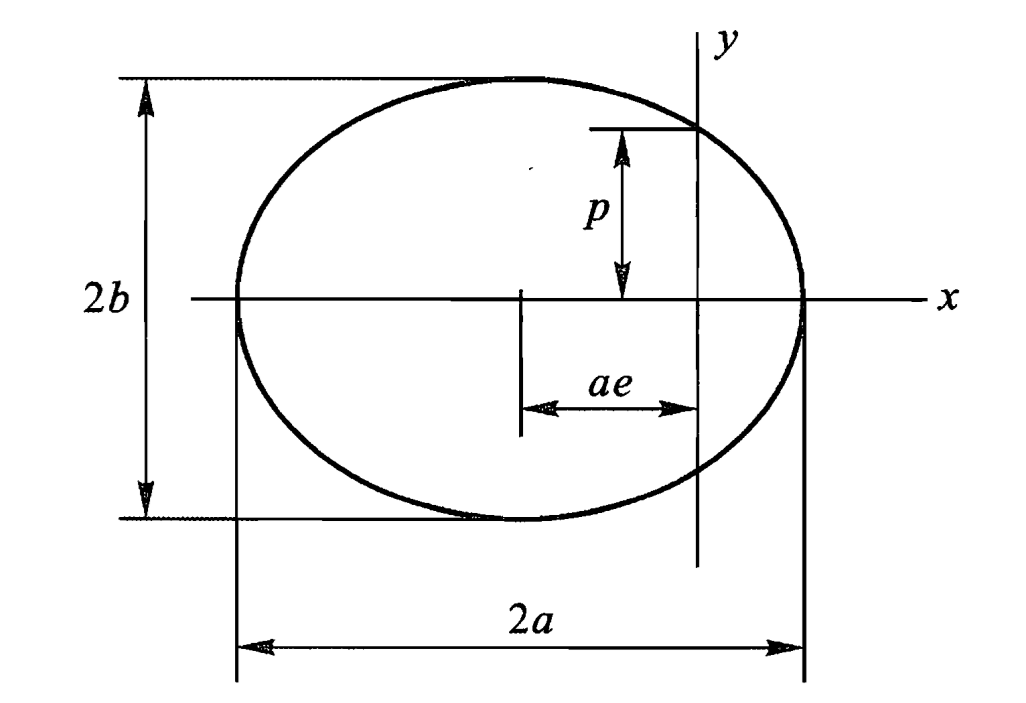
\includegraphics[height=3.5cm ,width=5cm]{CM/kepler1.png}
	\caption{Attractive Kepler orbit with $e < 1$}
\end{figure}\\
The major and minor semi-axes of the ellipse are
\[a = \frac{p}{1-e^2} = \frac{\alpha}{2|E|} \quad b = \frac{p}{\sqrt{1-e^2}} = \frac{M}{\sqrt{2m|E|}}\]
The least and greatest distances from the centre of the field (the focus of the ellipse) are
\[r_{min} = \frac{p}{1+e} = a(1-e) \quad r_{max} = \frac{p}{1-e} = a(1+e)\]
The period of revolution in an elliptical orbit is
\[T = \frac{\pi a b}{\frac{1}{2}r^2 \dot{\phi}} = 2\pi a^{3/2}\sqrt{\frac{m}{\alpha}} = \pi \alpha \sqrt{\frac{m}{2|E|^3}}\]
If $E > 0$, the path is a hyperbola with the origin as internal focus. 
\begin{figure}[!h]
	\centering
	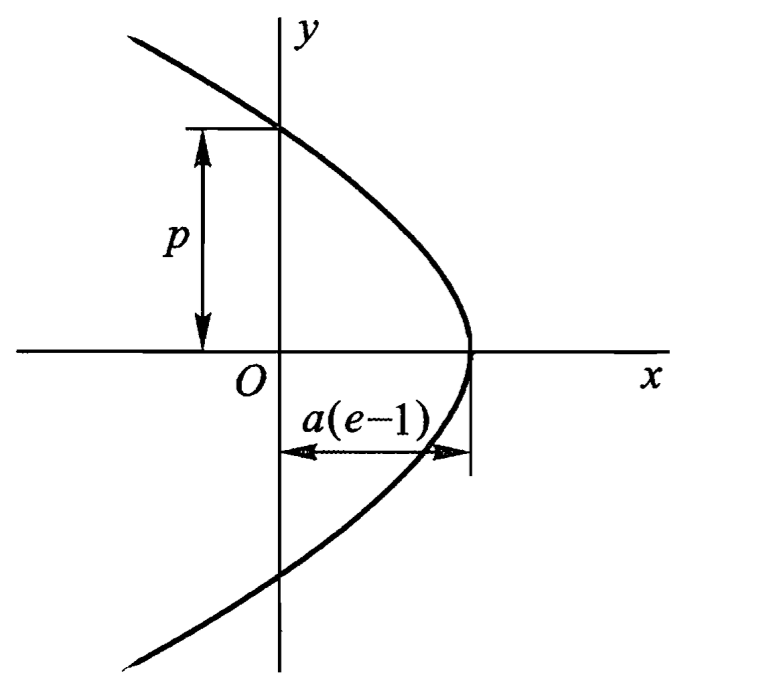
\includegraphics[height=3.5cm ,width=3.8cm]{CM/kepler2.png}
	\caption{Attractive Kepler orbit with $e > 1$}
\end{figure}\\
The distance of the perihelion from the focus is
\[r_{min} = \frac{p}{1+e} = a(1-e)\]
where $a = \frac{p}{(1-e^2)^2} = \frac{\alpha}{2E}$ is the semiaxis of the hyperbola.\\
If $E = 0$, the eccentricity $e = 1$, and the particle moves in a parabola with perihelion distance $r_{min} = \frac{p}{2}$. This case occurs if the particle starts from rest
at infinity.\\ \\
Let us now consider motion in a repulsive field, where
\[U= \frac{\alpha}{r} \quad (\alpha > 0)\]
Here the effective potential energy is
\[U_{eff} = \frac{\alpha}{r} + \frac{M^2}{2mr^2}\]
and decreases monotonically from $+\infty$ to zero as $r$ varies from zero to infinity. 
The energy of the particle must be positive, and the motion is always infinite. The calculations are exactly similar to those for the attractive field.
The path is a hyperbola:
\[\frac{p}{r} = -1 + e\cos\phi\]
\begin{figure}[!h]
	\centering
	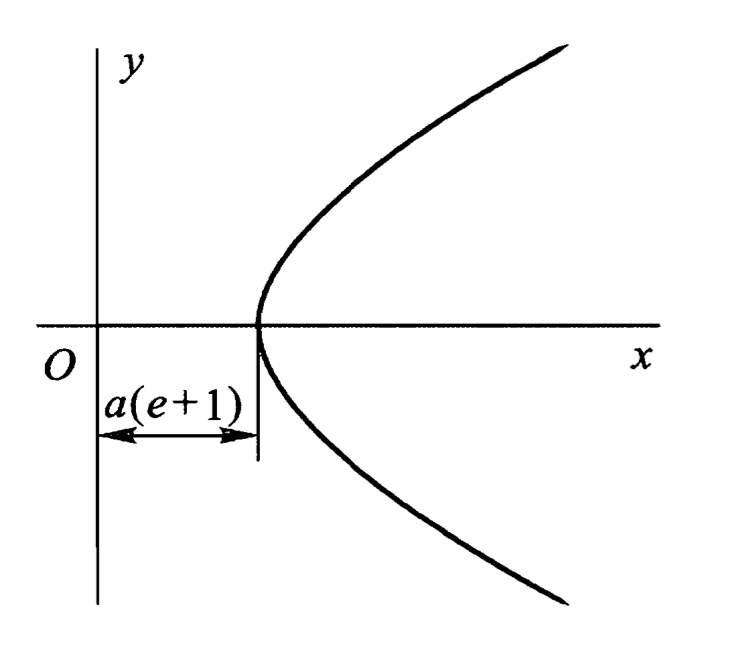
\includegraphics[height=3.3cm ,width=3.7cm]{CM/kepler3.png}
	\caption{Repulsive Kepler orbit}
\end{figure}\\
The perihelion distance is
\[r_{min} = \frac{p}{-1+e} = a(1+e)\]\\
There is an integral of the motion which exists only in fields $U = \frac{\alpha}{r}$. It is easy to verify by direct calculation that the quantity
\[\bm{v}\times\bm{M} + \frac{\alpha \bm{r}}{r}\]
is constant. The direction of the conserved vector is along the major axis from the focus to the perihelion, and its magnitude is $\alpha e$. This is most simply seen by considering its value at perihelion.

\section{Disintegration and collisions of particles}
Let us consider a spontaneous disintegration of a particle into two constituent parts. 
This process is most simply described in a frame of reference in which the particle is at rest before the disintegration.
The law of conservation of momentum shows that the sum of the momenta of the two particles formed in the disintegration is then zero; that is, the particles move apart with equal and
opposite momenta. The magnitude $p_0$ of either momentum is given by the law of conservation of energy:
\[E_i = E_{1i} + \frac{p_0^2}{2m_1} + E_{2i} + \frac{p_0^2}{2m_2}\]
here $m_1$ and $m_2$ are the masses of the particles, $E_{1i}$ and $E_{2i}$, their internal energies, and $E_{i}$ the internal energy of the original particle. If $\epsilon$ is the disintegration energy, i.e. the difference
\[\epsilon = E_i - E_{1i} - E_{2i}\]
which must obviously be positive, then
\[\epsilon = \frac{p_0^2}{2m}\]
here $m$ is the reduced mass of the two particles.\\
Let us now change to a frame of reference in which the primary particle moves with velocity $\bm{V}$ before the break-up. 
This frame is usually called the laboratory system, or L system, in contradistinction to the centre-of-mass
system, or C system, in which the total momentum is zero. 
Let us consider one of the resulting particles, and let $\bm{v}$ and $\bm{v}_0$ be its velocities in the L and
the C system-respectively. It can be represented by
\begin{figure}[!h]
	\centering
	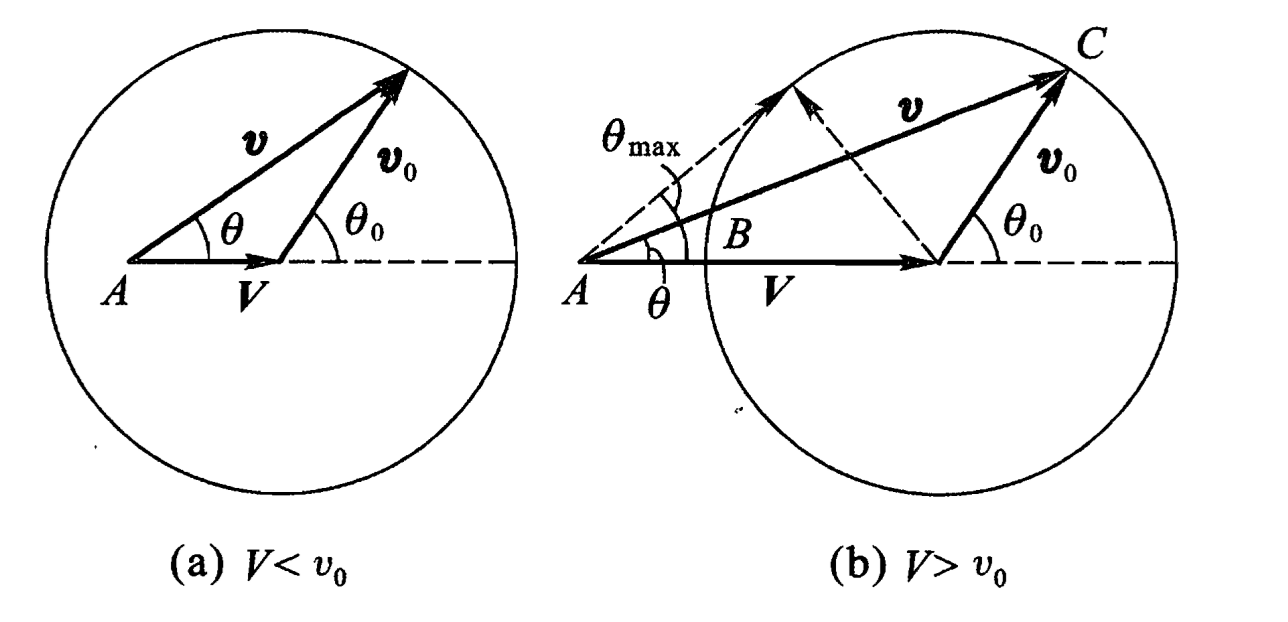
\includegraphics[height=4.5cm ,width=9.5cm]{CM/disintegration.png}
	\caption{Disintegration in L and C frame}
\end{figure}\\
The relation between the angles $\theta$ and $\theta_0$ in the L and C systems is evidently.
\[\tan\theta = \frac{v_0\sin\theta_0}{V+v_0\cos\theta_0}\]
In physical applications we are usually concerned with the disintegration of not one but many similar particles, and this raises the problem of the distribution of the resulting particles in direction, energy, etc. 
We shall assume that the primary particles are randomly oriented in space, i.e. isotropically on average.\\
In the C system, every resulting particle has the same energy, and their directions of motion are isotropically distributed. The fraction of particles entering a solid angle element $do$ is $\frac{do}{4\pi}$. 
So the distribution with respect to the angle $\theta_0$ is
\[\frac{1}{2}\sin\theta_0 d\theta_0\]
The corresponding distributions in the L system are obtained by an appropriate transformation. For example, let us calculate the kinetic energy distribution in the L system.
Since
\[v^2 = V^2 + v_0^2 + 2Vv_0\cos\theta_0\] 
we have $d(v^2) = d\cos\theta_0$. So the kinetic energy can distributed uniformly over between $T_{min} = \frac{1}{2}(v_0-V)^2$ and $T_{max}= \frac{1}{2}m(v_0+V)^2$.\\ \\
A collision between two particles is said to be elastic if it involves no change in their internal state. The collision is most simply described in the C system.The velocities of the particles before the collision are related to their velocities $\bm{v}_1$ and
$\bm{v}_2$ in the L system by $\bm{v}_{10} = m_2\bm{v}/(m_1+m_2)$, $\bm{v}_{20} = -m_1\bm{v}/(m_1+m_2)$,
where $\bm{v} = \bm{v}_1-\bm{v}_2$.\\
Because of the law of conservation of momentum, the momenta of the two particles remain equal and opposite after the collision, and are also unchanged in magnitude, by the law of conservation of energy. 
Thus, in the C system the collision simply rotates the velocities, which remain opposite in direction and unchanged in magnitude. The velocities of the two particles after the collision are
\[\bm{v}'_{10} = \frac{m_2v\bm{n}_0}{m_1+m_2} \quad \bm{v}'_{20} = -\frac{m_1v\bm{n}_0}{m_1+m_2}\]
The velocities in the L system after the collision are therefore
\[\bm{v}'_{1} = \frac{m_2v\bm{n}_0}{m_1+m_2} + \frac{m_1\bm{v_1}+m_2\bm{v_2}}{m_1+m_2} \quad \bm{v}'_{2} = -\frac{m_1v\bm{n}_0}{m_1+m_2} + \frac{m_1\bm{v_1}+m_2\bm{v_2}}{m_1+m_2}\]
Multiplying equations by $m_1$ and $m_2$ respectively, we obtain
\[\bm{p}'_{1} = mv\bm{n}_0 + \frac{m_1(\bm{p}_1 + \bm{p}_2)}{m_1+m_2} \quad \bm{p}'_{2} = -mv\bm{n}_0 + \frac{m_2(\bm{p}_1 + \bm{p}_2)}{m_1+m_2}\]
It can be represented by
\begin{figure}[!h]
	\centering
	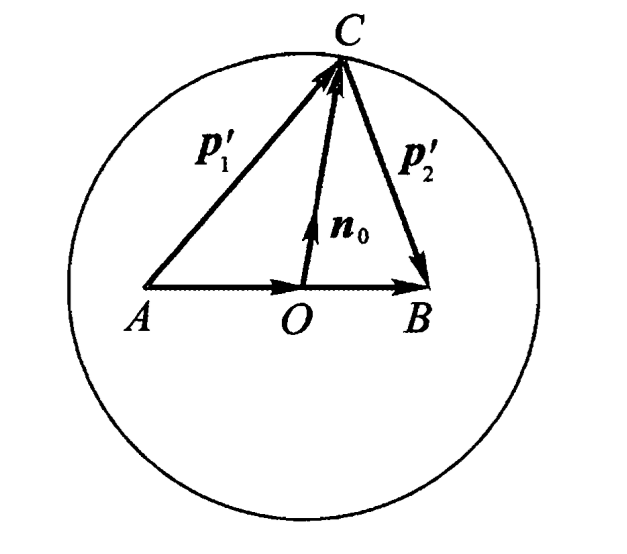
\includegraphics[height=3cm ,width=3.3cm]{CM/collision1.png}
	\caption{Collision in L and C frame}
\end{figure}\\
Let us consider in more detail the case where one of the particles ($m_2$, say) is at rest before the collision. In that case the distance $OB = \frac{m_2p_1}{m_1+m_2} = mv$ is equal to the radius. The vector $\vec{AB}$ is equal to the
momentum $\bm{p}_1$ of the particle $m_1$ before the collision.
\begin{figure}[!h]
	\centering
	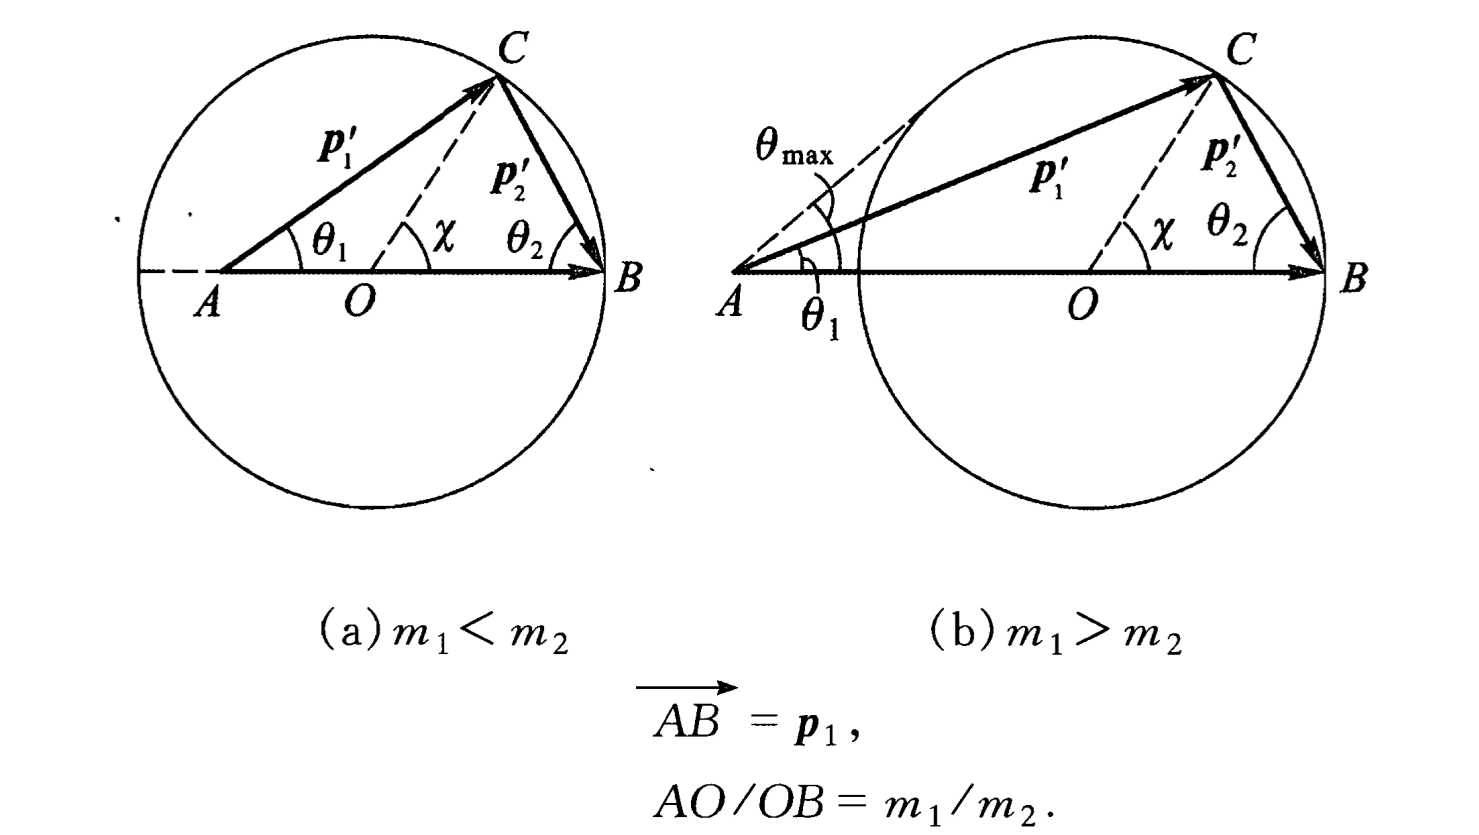
\includegraphics[height=4.2cm ,width=7.5cm]{CM/collision2.png}
	\caption{Collision with 2 at rest}
\end{figure}\\
$\theta_1$ and $\theta_2$ can be expressed in terms of $\chi$ by
\[\tan\theta_1 = \frac{m_2\sin\chi}{m_1 + m_2 \cos\chi} \quad \theta_2 = \frac{1}{2}(\pi - \chi)\]
The magnitudes of the velocities of the two particles after the collision in terms of $\chi$ are
\[v'_1 = \frac{\sqrt{m_1^2 + m_2^2 + 2m_1m_2\cos\chi}}{m_1+m_2}v \quad v'_2 = \frac{2m_1v}{m_1+m_2}\sin\frac{1}{2}\chi\]
If $m_1 < m_2$, the velocity of $m_1$ after the collision can have any direction.
If $m_1 > m_2$, this particle can be deflected only through an angle not exceeding $\theta_max$ from its original direction. Evidently
\[\sin\theta_{max} = \frac{m_2}{m_1}\]
The collision of two particles of equal mass, of which one is initially at rest, is especially simple. In this case both B and A lie on the circle, so
\begin{figure}[!h]
	\centering
	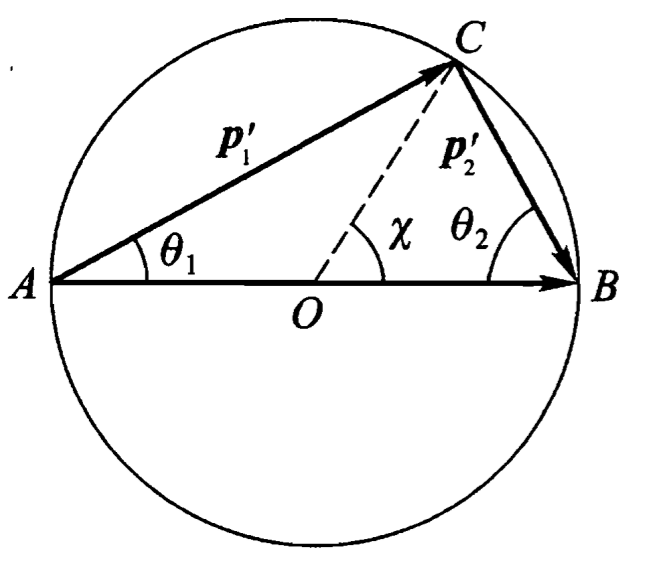
\includegraphics[height=2.9cm ,width=3.25cm]{CM/collision3.png}
	\caption{Collision of equal mass}
\end{figure}\\
Then 
\[\theta_1 = \frac{1}{2}\chi \quad \theta_2 = \frac{1}{2}(\pi-\chi)\]
\[v'_1 = v\cos\frac{1}{2}\chi \quad v'_2 = v\sin\frac{1}{2}\chi\]
After the collision the particles move at right angles to each other.
\end{document}